\section{Performance}
The overhead of both the SA and the GA are almost nothing ( $\le .01$ second per
iteration / generation). Especially compared to the cost / fitness function,
which has to run the simulation every time to get results. The main 
disadvantage of the GA over the SA is that for every iteration, it has to run
the simulation function once for every individual in the population. For this
project, the population size was 10, so the GA was approximately 10 times
as slow as the SA.

The good thing about the slowdown, is that it happens in data independent
region of the process; each fitness iteration for each individual can be 
calculated without needing to share data with other iterations. This meets the
criteria for true \textbf{task parallelism}, or running each fitness function
simultaneously.

\subsection{Enhancements with Parallelism}
To understand parallelism and the gains from it, we must consider Amdahl's Law:
\begin{figure}[h]
	\begin{center}
		\LARGE
		\begin{tabular}{l r}
			$ A $		&	$ = \frac{1}{(1 - P) + \frac{P}{N}} $ \\
		\end{tabular}

		\normalsize
		\begin{tabular}{l l}
			$ where $  & \\
					&	$ P $ is the portion of the program that can be 'parallelized' \\
					&	$ N $ processors or workers \\
					&	$ (1 - P) $ is the sequential / serial portion (cannot be parallelized) \\
		\end{tabular}
		\caption{Amdah's Law. \cite{amdahl}} 
		\label{amdahl}
	\end{center}
\end{figure}
\normalsize

$ P $ informally is the portion of the program that can be split up into sections, each of which can be worked 
on simultaniously. The name for this process is textbf{paralellization}. Informally, Ahmdahl's Law shows that 
the higher $ P $, or portion of work that can be split up, the more beneficial adding more CPU's ($ N $) is. Too many CPU's, and the benefit decreases.

For parallelism over many CPU's on a network, an API like OpenMPI can be used.
This creates an additional element, and that is the time cost of moving data
over the network:

\begin{figure}[h]
	\begin{center}
		\LARGE
		\begin{tabular}{l r}
			$ A $	&	$ = \frac{1}{((1 - P) + (T_P * N)) + \frac{P}{N}} $ \\
		\end{tabular}

		\normalsize
		\begin{tabular}{l l}
			$ where $  & \\
				&	$ P $ is the portion of the program that can be 'parallelized' \\
				&	$ N $ processors or workers \\
				&	$ (1 - P) $ is the sequential / serial portion (cannot be parallelized) \\
				&	$ (T_P * N) $ is the overhead \\
		\end{tabular}
		\caption{Amdah's Law (Figure \ref{amdahl}) with Overhead. } 
		\label{amdahl_overhead}
	\end{center}
\end{figure}
\normalsize

Adding more CPU's actual slows parallel processes down at a certain point.
For many algorithms, $ P $ can only be a fairly small size. The best value for $ N $ will then only be 1. If $ P $ is not very big to begin with, than any $ N $ greater than 1 will cause a slowdown instead 
of speedup. Thus, even though some programs can be parallelized, if $ N > 1 $ causes a slowdown, they shouldn't.

For the muscle excitation GA, we luckily have a fairly high $ P = 13.10 $
seconds,  and a low $ T_P = .08 $ seconds. $ P $ is the measured time for each
simulation to run, and $ T_P $ is an approximation of how long the data takes
to travel across an MPI network. The resulting graph for speed is below:

\begin{figure}[!h]
	\begin{center}
		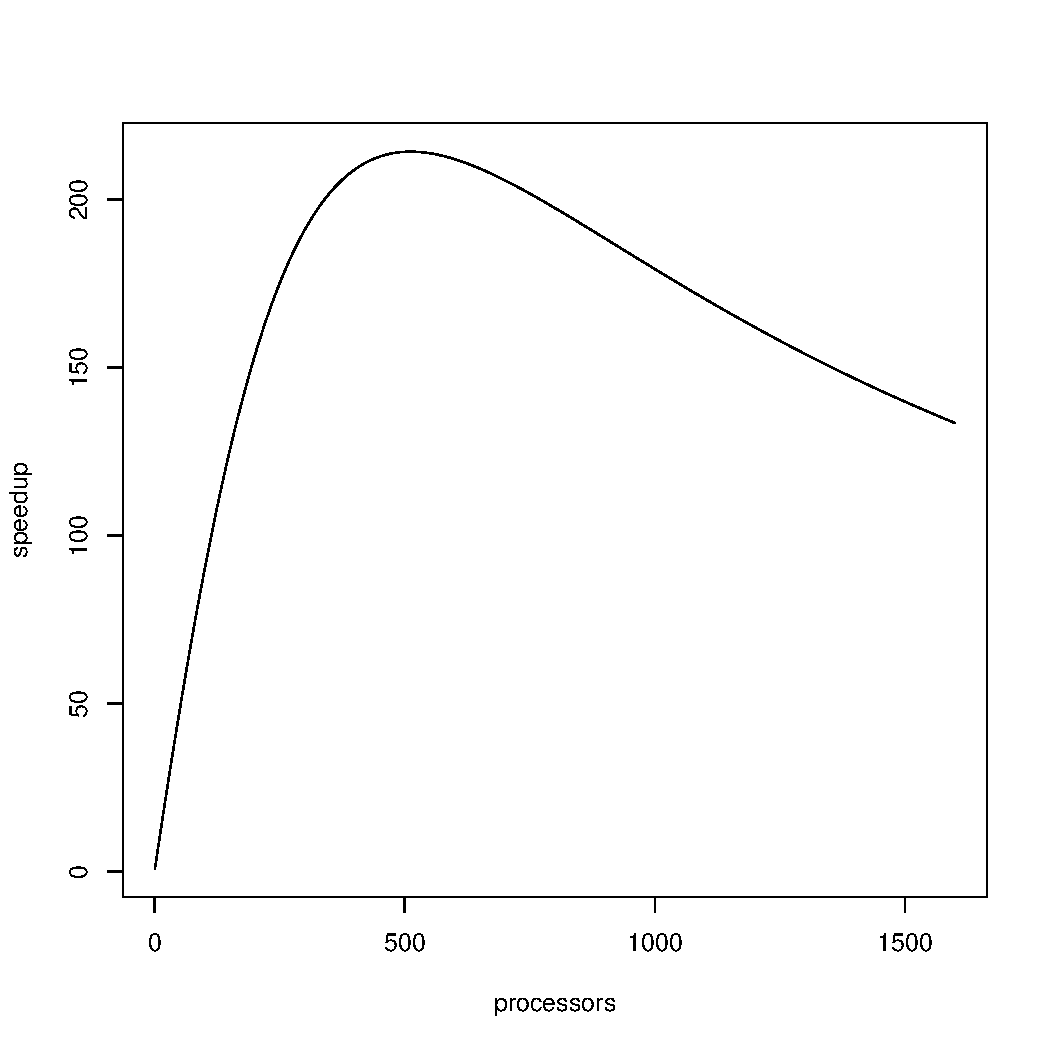
\includegraphics[width=120mm]{images/amdahl_graph.pdf}
               	\caption{Proposed speedup using OpenMPI and Amdahl's Law with Overhead (Figure \ref{amdahl_overhead}) }
                \label{speedup}
        \end{center}
\end{figure}

In figure \ref{speedup}, observe that the max speedup is 214.264919941776 with 
512 CPU's. Although this is the most speedup, significantly less will give more 
speedup for the extra cost, and a small to medium size computing cluster 
(50-100+ CPU's) would be very beneficial.

\section{Conclusion}
In conclusion, the GA outperformed the SA a little bit at the cost of a lot
of extra compute time. This may be still desirable, if the GA is in fact
exploring a global optimum. It is probable, however, that there is a very 
sudden global optimum somewhere, and this GA doesn't maintain enough diversity
to find it.

The project started with trying to imitate an SA using a GA, and then added 
more variability with mutation and crossover rates. What was quite suprising
was how sensitive the existing solution where to mutation and crossover.
The solutions the GA started with were recent bests found by the SA, and 
the GA originally changed them so much that fitness / cost went to infinity.
This is why this project used such conservative changes, scaling down 
mutations 800 times (Figure \ref{uniform_mutation}) and even leaving out 
crossover (Section \ref{sec:run_1}). When we did use crossover, it was very
conservative flip crossover, like flipping only 1, 2, or 3 attributes 
between individuals.

This conservation could be because the GA is already stuck in a local optimum,
and we have pressured it hard to not stray outside. It may also be that the 
fitness function is a little inaccurate.

In this report, it was hypothesized that the GA would find a better solution
through diversity. Instead, this GA found a better solution within the search
space that the SA was probably already searching. To get the GA to try more 
diverse solutions, it may be necessary to start the simulations without
initial solutions already found by the SA. We also hypothesized not much
performance difference between the SA and GA, but once we found out the
simulation time, this was definitely not true.

This GA found better solutions in our limited testing, but could probably
be better. Implementing the performance enhancements suggested may be the only
way to try larger populations, and to try more parameters for the GA.

Finally, it should be said that these parameters for the GA could easily be
controlled by another GA, or meta-GA. Even a GA for the fitness function
may be a good idea, as Dr. McGowan's current research edits this by hand.
There is a lot of opportunity for improvement, and hopefully some of the 
things found here will be useful in future research.
